\documentclass[10pt,a4paper,titlepage]{article}
\usepackage[utf8]{inputenc}

\usepackage{amsmath}
\usepackage{amsfonts}
\usepackage{amssymb}
\usepackage{graphicx}
\usepackage{float} % force figure to render inline location
\usepackage{enumitem} % apt install texlive-latex-extra 
\usepackage{anyfontsize} % custom fontsizes
\usepackage{titlesec} % custom section spacings
\usepackage{multirow} % merge table rows
\usepackage{vhistory} % revision table package

\setlist[itemize]{noitemsep} % No spaces in itemize lists
\setlist[enumerate]{noitemsep} % No spaces in itemize lists
\setlist[description]{noitemsep} % No spaces in itemize lists
\titlespacing*{\subsubsection}{0pt}{8pt}{2pt}
\titlespacing*{\paragraph}{0pt}{3pt}{5pt}

\newcommand{\cpright}{\textsuperscript{\tiny\copyright}}

\setlength\parindent{0pt}

\begin{document}
	
	\begin{titlepage}
		
		\title{
			\fontsize{50}{12}\selectfont{\textsc{Lunar Rover}}\\
			\vspace{20pt}
			\fontsize{20}{12}\selectfont{\textsc{Software Requirements Specification}}\\
			\vspace{10pt}
			\large{Software Engineering \& Project} \\
			\vspace{20pt}
			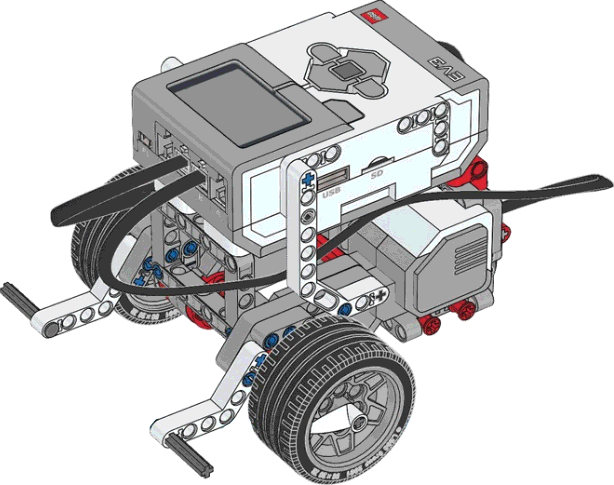
\includegraphics[width=200px]{title-page-ev3.png}					
		}
		\date{20/08/2017}
		\author{
			\bf{Team: PG-29} \\
			Benjamin Winding \\
			Kin Leong Lee \\
			Pavitterjeet Sidhu \\
			Phan Huy Nguyen \\
			Sean Hennessy \\
			Xiaoshan Chen \\
		}
		\maketitle
		
	\end{titlepage}
		 
	\tableofcontents	
	\listoffigures
	
	
	\section*{Revision History}	
	\label{revtable}	
	\begin{tabular}{|p{2.1cm}|p{2.5cm}|p{2cm}|p{4.1cm}|}		
		\hline 
		\textbf {Name} & \textbf{Date} & \textbf {Version} &\textbf {Summary of Changes} \\ 
		\hline 
		1st Draft & 21/08/2017 & 1.0 & Initial Draft\\
		\hline
		2nd Draft & 27/08/2017 & 2.0 & Identificatons numbers added. Grammar improvements. Diagrams revisisted. Assumptions added. Priority classifications Added.\\ 
		\hline 		
	\end{tabular}

	\newpage
	
	\section{Introduction}
	\subsection{Purpose}
	This report is to describe the software requirements specification of the lunar rover project. The lunar rover project involves building a prototype rover capable of surveying a designated area automatically. The project is to be completed in semester 2 2017.
	
	\subsection{Document Conventions}
	This document contains a series of user requirements. These requirements have been broken down into categories and given a priority based on the sequence they are stated, the first being the most important feature.
	\paragraph{}
	Acronyms are also prevalent in the document. These mainly consist of computer technology acronyms such as:
	\begin{description}[align=right,labelwidth=3cm]
		\item [App] Application
		\item [GUI] Graphical User Interface
		\item [SRS] Software Requirements Specification 
		\item [....]
	\end{description}
	
	\subsection{Intended Audience and Reading Suggestions}
	The intended audience of this document are the Client, this project team and project supervisor. Reading suggestions for this document are:
	\begin{itemize}
		\item Client Specification
		\item Project Specification
		\item LEGO\cpright Mindstorms EV3 kit overview
		\item LeJOS EV3 Java Library overview
	\end{itemize}
	
	\subsection{Project Scope}
	\paragraph{}
	The scope of this project is to demonstrate a prototype for a lunar robot, which is capable of performing an automated survey of a extraterrestrial landscape.
	\paragraph{}
	This robot is to be constructed using the EV3 LEGO\cpright Mind-storms robot provided by the client. It is to be controlled via a remote location, but is required to automatically make decisions based on the environment around it.
	
	\subsection{References}
	1. Client Specifications, \\
	2. Project Specifications, \\
	3. Ev3 kit
	
	\section{Overall Description}
	\subsection{Product Perspective}
	The product described in this SRS is a self-contained project. It relies on the existing LEGO\cpright Mindstorms robot, supplied by the client. Previously, the robot cannot be controlled by a human being with software no matter whether manually or automatically. This SRS defines the component of the robot system and the following diagram is identifying the functionalities and interfaces of this system.
	
	\begin{figure}[H]
		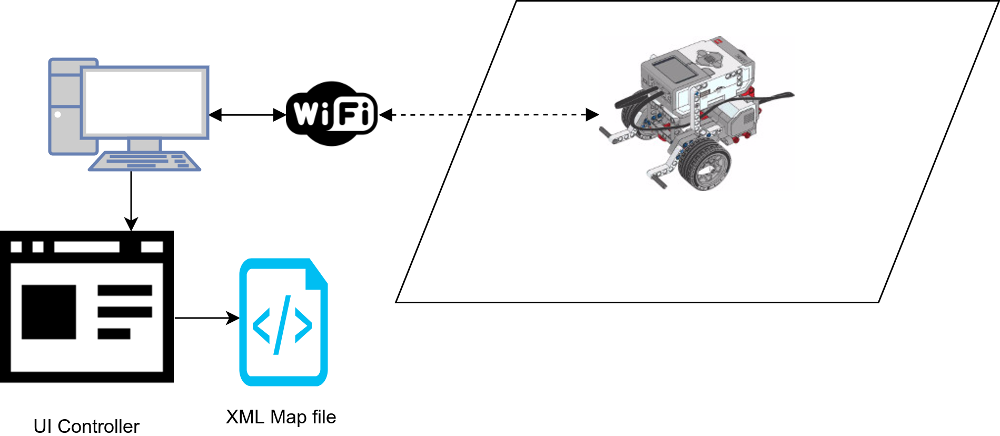
\includegraphics[width=\linewidth]{Robot_system.png}  % created using www.draw.io
		\caption{High level system overview}
		\label{fig:system overview}				
	\end{figure}
	
	\subsection{Product Features}
	The main features of this robot include
	\begin{itemize}
		\item Automatic survey of specified areas
		\item Remote control manual override and movement
		\item On-board obstacle avoidance mechanisms 
		\item No-go zone detection and avoidance
		\item Ability to return to the starting point or any point selected on mapped area.
	\end{itemize}
	
	\subsection{User Classes and Characteristics}
	\paragraph{}
	The users of the robot include three types; the client, students and teachers. All users must read the user documentation and safety material before operating the robot.
	\paragraph{}
	The client is the primary user of the final system. However during development the client may be able to request test runs of the robot, only after reading the relevant user documentation.
	\paragraph{} 
	Students include project group members and those students enrolled in the university of Adelaide. Students must given explicit permission to use the system by a teacher or project group member.
	\paragraph{}
	Teachers who have been granted permission to use the system must be familiar with the GUI control and safety precautions prior to using the system. 
	
	\subsection{Operating Environment}
	The software can be run on Windows, Mac or Ubuntu systems, specific details are shown in fig \ref{fig:tab Os Requirements}. WiFi access is required to run the control software. Additionally the GUI must be compiled using JDK (version 1.7 only).
	
	\begin{figure}
		\centering
		\begin{tabular}{|p{2cm}|p{2cm}|p{7cm}|}
			\hline 
			\textbf{OS} &\textbf{Minimum Version} & \textbf{Requirements} \\ 
			\hline 
			Windows & 7 & 1 (GHz) or faster 32-bit (x86) or 64-bit (x64) processor*;
			1 gigabyte (GB) RAM (32-bit) or 2 GB RAM (64-bit);
			16 GB available hard disk space (32-bit) or 20 GB (64-bit);
			DirectX 9 graphics device with WDDM 1.0 or higher driver. \\ 
			\hline 
			Mac & OS X 10 & An Intel Core 2 Duo, Core i3, Core i5, Core i7, or Xeon processor;
			7 GB of available disk space;
			2 GB of RAM. \\ 
			\hline 
			Ubuntu & 16.10 & 1 (GHz) or faster 32-bit (x86) or 64-bit (x64) processor*;
			1 gigabyte (GB) RAM (32-bit) or 2 GB RAM (64-bit);
			16 GB available hard disk space (32-bit) or 20 GB (64-bit); \\
			\hline 
		\end{tabular} 
		\caption{Detailed operating system requirements}
		\label{fig:tab Os Requirements}
	\end{figure}
	
	\subsection{Design and Implementation Constraints}
	\subsubsection*{Implementation Constraints}
	The system is to be implemented using the EV3 LEGO\cpright Mindstorms kit supplied by the client. The embedded software on the rover is to be written in Java, using the LeJOS Ev3 library version:0.9.0. And the external code used in the system shall not exceed 10\%. The build tool for compiling the software and deploying it to the system is \textit{ant}. The system will be implemented using the wireless technology WiFi over an encrypted WPA2 connection.
	
	\subsubsection*{Development Constraints}
	The university enterprise Github instance is the version control system to be used throughout the project. During development the project team will use the IntelliJ IDE to design and write code. Slack is used for communication and coordination through out the project. Lastly, Latex is used to produce documentation since it is simple and is easier to maintain in a version control system.
	
	\subsection{User Documentation}
	At the end of the project, a user manual will be available to users via a handbook. The handbook will mainly describe the different parts of GUI, including the getting started window, the paths and targets browser, the off-line and online browser and so on, assisting users to control the robot better.
	
	\subsection{Assumptions and Dependencies}
	
	It is assumed that the password is entered correctly and the robot establishes connection successfully with appropriate software and hardware. Also, the robot is ready to be control manually or automatically. \\ 

	Additional assumptions and dependencies include: 
	\begin{itemize}
		\item The robot is controlled in manual mode before in automagical mode
		\item The volume of battery is enough to support the robot throughout the survey
		\item Each member of this project are expected to spending 120 hours completing the project
		\item The robot will not surrounded by the NGZ
		\item Everyone will complete the assigned sections 
		\item Any area within the map can be landing zones, excluding NGZ's
		\item The map clearly shows the colours of track/trails
		\item The map is flat surface
		\item The map is rectangular
		\item NGZ's will not be manually entered during the survey.
		\item Thickness of the line is no less than 1.5cm
		\item Trail lines are reasonably smooth, no crossing paths
	\end{itemize}
	
		\section{User Requirements}
	\subsection{The Map}
    \begin{itemize}
		\item \textbf{UR01:} The robot shall enter the survey area and produce a survey map
		\begin{itemize}
			\item \textbf{Priority:} High
            \item \textbf{Dependency:} None
			\item \textbf{Description:} Upon landing, the robot shall enter the survey area and produce a survey map based on the track followed by the vehicle. 
            \item \textbf{Rationale:} This map will be used to analyze the survey area. This map will also be used to monitor and provide instruction to the vehicle.  
            \item \textbf{Acceptance criteria:} This requirement can be verified by doing a survey of an area  by using the software that we are going to develop and the survey map will be automatically produced. 
		\end{itemize} 
	\end{itemize}
    
    \begin{itemize}
		\item \textbf{UR02:} The map shall be constructed in real time
		\begin{itemize}
			\item \textbf{Priority:} High
            \item \textbf{Dependency:} UR01
			\item \textbf{Description:} After landing the robot on the predefined landing zone, the map shall be constructed in real time as long as the robot starts the survey. 
            \item \textbf{Rationale:} This feature will allow the remote operator to monitor and instruct the robot in real time. 
            \item \textbf{Acceptance criteria:} This requirement can be verified by physically observing the robot and comparing the changes on the map. 
		\end{itemize} 
	\end{itemize}
    \begin{itemize}
		\item \textbf{UR03:} The map shall allow to designate NGZ any time
		\begin{itemize}
			\item \textbf{Priority:} High
            \item \textbf{Dependency:} None
			\item \textbf{Description:}  The remote operate shall be able to designate NGZ any time on the map by using the GUI of the software. 
            \item \textbf{Rationale:} This feature can be very useful in avoid any potential dangerous areas of the map detected by the remote operator. 
            \item \textbf{Acceptance criteria:} This requirement can be verified by drawing a few NGZ on a sample map using GUI. 
		\end{itemize} 
	\end{itemize}
	\begin{itemize}
		\item \textbf{UR04:} The current location of the vehicle shall be visible on map
		\begin{itemize}
			\item \textbf{Priority:} Medium
            \item \textbf{Dependency:} UR02
			\item \textbf{Description:}  The current location of the vehicle shall be clearly visible on the map in real time. No matter where the robot goes in the map, the operator shall be able to track the current location.  
            \item \textbf{Rationale:} This feature will allow the remote operator to track the current location of the robot.   
            \item \textbf{Acceptance criteria:} This requirement can be verified by moving the robot into different directions and physically comparing the actual position of the robot between the physical map and the map on the GUI. 
		\end{itemize} 
	\end{itemize}
    \begin{itemize}
		\item \textbf{UR05:} The map shall be able to be stored in "XML" format
		\begin{itemize}
			\item \textbf{Priority:} Medium
            \item \textbf{Dependency:} UR01
			\item \textbf{Description:} The survey map which shall be created during the process of survey, shall be able to be stored in "XML" format in the system.  
            \item \textbf{Rationale:} This feature will allow the user to store, process, share etc. the survey map. 
            \item \textbf{Acceptance criteria:} This requirement can be verified by storing any sample survey map in "XML" format and then viewing it in "XML" supported platform only. 
		\end{itemize} 
	\end{itemize}
    \begin{itemize}
		\item \textbf{UR06:} The software shall allow to load existing "XML" map file
		\begin{itemize}
			\item \textbf{Priority:} Low
            \item \textbf{Dependency:} None
			\item \textbf{Description:} The user shall be able to load any existing partial or fully completed survey map file in "XML" format into the software. 
            \item \textbf{Rationale:} This feature will allow the user to test the robot before sending it to actual survey area and will also be handy in case of system failure. 
            \item \textbf{Acceptance criteria:} This requirement can be verified by loading an exiting "XML" map file in the software and by allowing the robot to survey this map.  
		\end{itemize} 
	\end{itemize}
    \begin{itemize}
		\item \textbf{UR07:} The map shall allow to zoom in on particular area
		\begin{itemize}
			\item \textbf{Priority:} Low
            \item \textbf{Dependency:} None
			\item \textbf{Description:} The user shall be able to zoom in on particular area in the map by using the GUI of the software.  
            \item \textbf{Rationale:} This feature can be very useful if the user wants to focus on a particular area on the map and wants to have a closer and detailed look.  
            \item \textbf{Acceptance criteria:} This requirement can be verified by client by zooming in on a particular area of a sample map.  
		\end{itemize} 
	\end{itemize}
    
	\subsection{Sensors}
  
    \begin{itemize}
		\item \textbf{UR08:} The robot shall detect craters
		\begin{itemize}
			\item \textbf{Priority:} High
            \item \textbf{Dependency:} None
			\item \textbf{Description:} The robot shall detect and avoid going into carters during the survey and try to find an alternate route to destination. 
            \item \textbf{Rationale:} This feature will protect the robot from going into area where it is impossible for robot to recover without assistance. 
            \item \textbf{Acceptance criteria:} This requirement can be verified by trying to send the robot into craters by setting the destination on other side of the carter. 
		\end{itemize} 
	\end{itemize}  
    \begin{itemize}
		\item \textbf{UR09:} The robot shall not collide against an external object
		\begin{itemize}
			\item \textbf{Priority:} High
            \item \textbf{Dependency:} None
			\item \textbf{Description:} The robot shall detect an external object and avoid colliding with it . 
            \item \textbf{Rationale:} This feature will protect the expensive vehicle from harm and also preserve the integrity of the survey site. 
            \item \textbf{Acceptance criteria:} This requirement can be verified by instructing the robot to move towards an external object. 
		\end{itemize} 
	\end{itemize}
	\begin{itemize}
		\item \textbf{UR10:} The robot shall not go into any NGZ on map
		\begin{itemize}
			\item \textbf{Priority:} High
            \item \textbf{Dependency:} None
			\item \textbf{Description:} The robot shall detect and avoid going into any NGZ available on the survey map. 
            \item \textbf{Rationale:} NGZ is considered as potentially dangerous area of the map in which robot shall not go. By doing so, the robot can be protected from any harm.  
            \item \textbf{Acceptance criteria:} This requirement can be verified by trying to send the robot into NGZ by setting the destination of the robot on other side of the NGZ.  
		\end{itemize} 
	\end{itemize}
    \begin{itemize}
		\item \textbf{UR11:} The robot shall be able to detect a track on a given map
		\begin{itemize}
			\item \textbf{Priority:} Medium
            \item \textbf{Dependency:} None
			\item \textbf{Description:} The robot shall be able to detect and follow any given track on the survey map.  
            \item \textbf{Rationale:} This will allow the operator to survey the specific area of the map. 
            \item \textbf{Acceptance criteria:}  This requirement can be verified by loading an existing survey map with at least one track into software and robot will detect and follow that track. 
		\end{itemize} 
	\end{itemize}
	
	\subsection{Operations}
   
    \begin{itemize}
		\item \textbf{UR12:} The robot shall be able to move immediately to a given point
		\begin{itemize}
			\item \textbf{Priority:} High
            \item \textbf{Dependency:} None
			\item \textbf{Description:} The remote operator shall be able to place survey point on the map and the robot shall move immediately towards that point. 
            \item \textbf{Rationale:}  This feature will allow the operator to survey any area on the map by just setting the survey point on the map.
            \item \textbf{Acceptance criteria:}  This feature can be verified by setting a survey point on the map using the GUI and the robot will move towards it. 
		\end{itemize} 
	\end{itemize}
    \begin{itemize}
		\item \textbf{UR13:} The operator shall be able to stop the robot at any time
		\begin{itemize}
			\item \textbf{Priority:} High
            \item \textbf{Dependency:} None
			\item \textbf{Description:} The remote operator shall be able to stop the robot at any time using the stop button on the GUI.
            \item \textbf{Rationale:} This feature can be useful in protecting the robot or if the operator wants to abort the mission, he/she can just stop the robot and instruct it to return to the landing site.  
            \item \textbf{Acceptance criteria:} This requirement can be verified by pressing the stop button on GUI and in response to this, the robot will stop immediately. 
		\end{itemize} 
	\end{itemize} 
     \begin{itemize}
		\item \textbf{UR14:} The software shall provide manual control of the robot as well
		\begin{itemize}
			\item \textbf{Priority:} Medium
            \item \textbf{Dependency:} None
			\item \textbf{Description:}  The operator shall be able to take manual control of the robot at any time.   
            \item \textbf{Rationale:} This feature can be useful in manually adjusting the position of the robot at any time. 
            \item \textbf{Acceptance criteria:} This requirement can be verified controlling the robot manually at any time using the provided GUI. 
		\end{itemize} 
	\end{itemize}
    \begin{itemize}
		\item \textbf{UR15:} The robot shall return to landing site
		\begin{itemize}
			\item \textbf{Priority:} Medium
            \item \textbf{Dependency:} None
			\item \textbf{Description:} The robot shall remember its landing site and shall return to it when the survey is finished.
            \item \textbf{Rationale:}  This feature will allow the operator to bring the robot back, once the survey is finished.
            \item \textbf{Acceptance criteria:} This requirement can be verified by instructing the robot to return to the landing site at any time during the survey. 
		\end{itemize} 
	\end{itemize}
   
	
	\section{System Features}
	\subsection{Map input feature}
	This feature is designed to allow the operator to manually enter new information to the map such as NGZ, start/destination point, tracks/trails.
	
	\subsubsection*{Stimulus}
	\begin{enumerate}
		\item Open MJ Control application.
		\item Enter username/password.
		\item Click button “Add map info”.
		\item Select information type from info type drop-down list (NGZ, tracks/trails etc.)
		\item Click on the map to input new map information.
		\item Click “Save”/”Cancel” to save or discard map information.
	\end{enumerate}
	
	\subsubsection*{Response}
	\begin{itemize}
		\item Save new information enter by operator into map XML file.
	\end{itemize}
	
	\subsubsection*{Functional requirements}
	\begin{itemize}
		\item \textbf{FR001} 
		\begin{itemize}
			\item \textbf{Priority:} High
			\item \textbf{Dependency:} None
			\item \textbf{Description:} The application provides a UI to enter new map information.
		\end{itemize}
		\item \textbf{FR002}
		\begin{itemize}
			\item \textbf{Priority:} High
			\item \textbf{Dependency:} None
			\item \textbf{Description:} The application shall translate new map information into correct XML format and update current XML map info file with new information.
		\end{itemize}
	\end{itemize}
	
	\subsection{Map imported/exported feature}
	This feature designed to allow operator to import a predefine map or export current map information in XML format.
	
	\subsubsection*{Stimulus}
	\begin{enumerate}
		\item Open MJ Control application.
		\item Enter username/password.
		\item 
		\begin{enumerate} 
			\item \textbf{For import action:} Click “Import map” browse to existed XML map file.
			\item \textbf{For export action:} Click” Export map” system will automatically generate latest XML map information with unique name (Map-export-[current-time].xml) in “MapExport” folder of application.
		\end{enumerate} 
	\end{enumerate}
	
	\subsubsection*{Response}
	\begin{itemize}
		\item Load imported map to the UI screen.
		\item Save latest info to “MapExport” folder when operator click export.
	\end{itemize}
	
	\subsubsection*{Functional requirements}
	\begin{itemize}
		
		\item \textbf{FR003} 
		\begin{itemize}
			\item \textbf{Priority:} High
			\item \textbf{Dependency:} None
			\item \textbf{Description:} The application shall allow operator import initial map information at the beginning of the survey mission. The application shall disable import button while robot is surveying the map.
		\end{itemize}
	
		\item \textbf{FR004} 
		\begin{itemize}
			\item \textbf{Priority:} High
			\item \textbf{Dependency:} None
			\item \textbf{Description:} The application shall allow operator export map information and save it with a unique name in designated folder.
		\end{itemize}
	\end{itemize}
	
	\subsection{Map display feature}
	This feature is designed to display information of survey area in real-time and robot location. This feature also allow operator to import a XML partial map. The operators can see completed map information with zoom-in/zoom-out supported. Map will display information from imported map, manual input information from operator and real-time information return from robot while it explores the survey area (obstacle, tracks/trail, radiation area etc.)
	
	\subsubsection*{Stimulus}
	\begin{enumerate}
		\item Open MJ Control application.
		\item Enter username/password.
		\item (optional): Use “import map” button to browse to existing XML predefined map if there is one.
		\item (optional): Use manual control mode or autonomous to explore survey area.
		\item (optional): Use “Map input” feature to manual add new information to map.
		\item (optional): Zoom-in/Zoom-out on a specific region.  
	\end{enumerate}
	
	\subsubsection*{Response}
	\begin{itemize}
		\item Realtime information displays on GUI map.
	\end{itemize}
	
	\subsubsection*{Functional requirements}
	\begin{itemize}
		
		\item \textbf{FR005} 
		\begin{itemize}
			\item \textbf{Priority:} High
			\item \textbf{Dependency:} None
			\item \textbf{Description:} The application shall allow to import predefined a xml format map file which comply with predefine DTD provide by client.
		\end{itemize}
		\item \textbf{FR006} 
		\begin{itemize}
		\item \textbf{Priority:} Normal
		\item \textbf{Dependency:} FR005
		\item \textbf{Description:} The application shall display all information from imported map, operator inputs and survey info return from robot at real-time.
		\end{itemize}
	
	\end{itemize}
	
	\subsection{Manual control feature }
	This feature designated to allow operator manual control robot. It also has function to switch between manual/autonomous control and emergency stop.
	
	\subsubsection*{Stimulus}
	\begin{enumerate}
		\item Open MJ Control application.
		\item Enter username/password.
		\item Use navigation button on UI to control robot.
		\item Switch between Autonomous/Manual control by turn on/off “Autonomous Control” toggle button.
		\item Emergency stop robot by click “Emergency Stop” button
	\end{enumerate}
	
	\subsubsection*{Response}
	\begin{itemize}
		\item Robot moving correct when operator use navigation buttons in manual control mode.
		\item When click on autonomous mode all navigation buttons will be disabled and robot will autonomous survey the area with internal survey algorithm.
		\item Emergency stop will stop robot intermediately both on manual/autonomous mode.
	\end{itemize}
	
	\subsubsection*{Functional requirements}
	\begin{itemize}
		
		\item \textbf{FR008} 
		\begin{itemize}
			\item \textbf{Priority:} High
			\item \textbf{Dependency:} FR006
			\item \textbf{Description:} The application shall allow operator manual control robot precisely with navigation buttons.
		\end{itemize}
		\item \textbf{FR009} 
		\begin{itemize}
		\item \textbf{Priority:} High
		\item \textbf{Dependency:} None
		\item \textbf{Description:} Emergency stop button shall stop robot immediately navigation buttons.
		\end{itemize}
	
		\item \textbf{FR010} 
		\begin{itemize}
			\item \textbf{Priority:} High
			\item \textbf{Dependency:} None
			\item \textbf{Description:} The application shall allow switch between manual/autonomous mode.
		\end{itemize}
	
		\item \textbf{FR011} 
		\begin{itemize}
			\item \textbf{Priority:} Normal
			\item \textbf{Dependency:} FR006
			\item \textbf{Description:} While robot move under manual control. All map information collected from sensor will be recorded and display on map as describe feature 4.3.
		\end{itemize}
	\end{itemize}
	
	
	\subsection{Autonomous control feature }
	Robot have ability to self-control and autonomously survey the area. Robot also can auto navigate from one point to another point on the map after get instruction from operator.
	
	\subsubsection*{Stimulus}
	\begin{itemize}
		\item Step 1: Open MJ Control application.
		\item Step 2: Enter username/password.
		\item Step 3: Step 3: Click the Autonomous Control” toggle button to turn on autonomous mode.
		\item Step 4 (optional): Click on “Move to Location” button and enter the destination coordinate (x,y). Robot will auto navigate from current location to entered destination.
	\end{itemize}
	
	\subsubsection*{Response}
	\begin{itemize}
		\item Robot will self-control and autonomously survey area then move back to landing point after mission completed. While in autonomous mode all navigation buttons will be disabled.
	\end{itemize}
	
	\subsubsection*{Functional requirements}
	\begin{itemize}
		
		
		\item \textbf{FR012} 
		\begin{itemize}
			\item \textbf{Priority:} High
			\item \textbf{Dependency:} FR004
			\item \textbf{Description:} The application shall have an self-control module which can control and navigate robot automatically corresponding to information from the map and sensors data while surveying.
		\end{itemize}
		\item \textbf{FR013} 
		\begin{itemize}
		\item \textbf{Priority:} High
		\item \textbf{Dependency:} None
		\item \textbf{Description:} The application shall have an obstacle detection algorithms that prevent robot collide with obstacle or move into NGZ's/Craters.
		\end{itemize}
	
		\item \textbf{FR014} 
		\begin{itemize}
			\item \textbf{Priority:} Normal
			\item \textbf{Dependency:} FR013
			\item \textbf{Description:} The application shall have a build in algorithm to find the safe and shortest path to navigate from one location to another location.
		\end{itemize}
		\item \textbf{FR011}
	
	\end{itemize}
	
	\subsection{Authentication feature }
	\text This feature is designed to prevent un-authorised persons from accessing control of the robot.
	
	\subsubsection*{Stimulus}
	\begin{enumerate}
		\item Open MJ Control application.
		\item Enter username/password.
	\end{enumerate}
	
	\subsubsection*{Response}
	\begin{itemize}
		\item Grant access to MJ control UI if username/password valid. Otherwise, display un-authorisation message
	\end{itemize}
	
	\subsubsection{Functional requirements}
	\begin{itemize}
		\item \textbf{FR015}
		\begin{itemize}
			\item \textbf{Priority:} Normal
			\item \textbf{Dependency:} None
			\item \textbf{Description:} Application shall provide authentication step before operator can start to control robot.
		\end{itemize} 
		
	\end{itemize}
	
	\section{External Interface Requirements}
	\subsection{User Interfaces}
	Graphic User Interface will be provided to allow a user to interact with the system through graphical buttons and map scene. The size of GUI shall be large enough to display system message and map information clearly. This GUI will be implemented by using JavaFX. There are three types of buttons and two types of display area. The specific details of the user interface design will be documented in a separate user interface specification. 
	
	\begin{figure}[H]
		\centering
		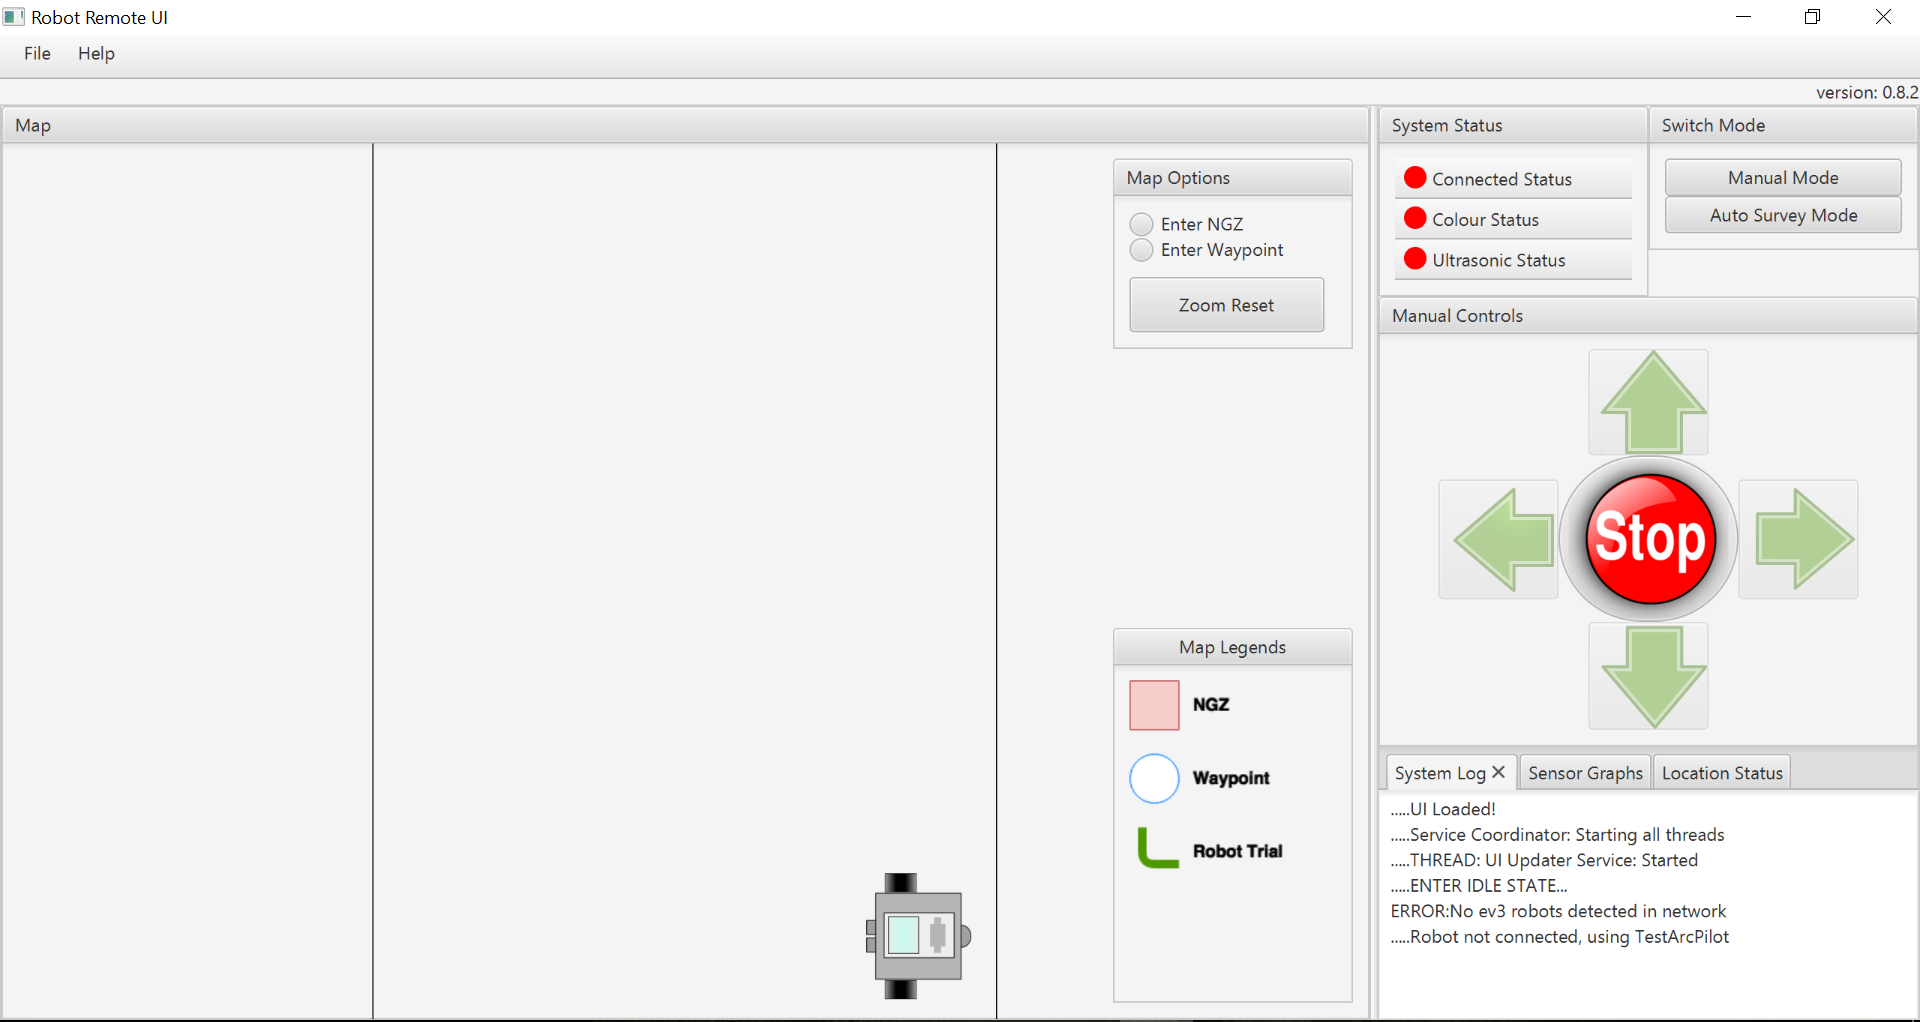
\includegraphics[width=300px]{GUI.PNG}
		\caption{The prototype of GUI with keyboard shortcuts for each button}
		\label{fig:GUI with keyboard shortcuts}
	\end{figure}
	
	\subsubsection*{EIR01: Button Functions}
	\paragraph{Priortiy:} High
	\paragraph{Dependencies:} UR05, UR06, UR14
	\paragraph{Description:} GUI shall provide a set of buttons for an user to coontrol the robot and perform the features which are describled in section 3. The following is the table to illustrate the functionalities for each button.

	\begin{figure}[H]
		\centering
		\begin{tabular}{|p{3cm}|p{6cm}|}
			\hline 
			\textbf{Button} &\textbf{Action} \\ \hline 
			Up & Robot moves forward \\ \hline 
			Left & Robot makes a left turn \\ \hline 
			Right & Robot makes a right turn \\ \hline 
			Down & Robot moves backward \\ \hline 
			Connect & Establish connection to remote robot \\ \hline 
			Disconnect & Disconnect from remote connection \\ \hline 
			Switch Mode & Switch the current mode of the robot. If the robot is in Navigation mode then change the robot to Auto mode, and vice versa. \\ \hline 
			Upload & Upload partially complete map data to the system \\ \hline
			Download & Save the current map information to a local XML file \\ \hline
		\end{tabular} 
		\caption{Buttons functions during manual remote control}
		\label{fig:button functions manual}
	\end{figure}

	\subsubsection*{EIR02: Map panel}
	\paragraph{Priortiy:} High
	\paragraph{Dependencies:} UR05, UR06, UR14
	\paragraph{Description:} The map information component provides a user interface to view and interact with the map in real time.
	
	\begin{figure}[H]
		\centering
		\begin{tabular}{|p{3cm}|p{6cm}|}
			\hline 
			\textbf{Button} &\textbf{Action} \\ \hline 
			Mouse Click & Draws a visual NGZ on the map\\ \hline 
			Scroll wheel & Zooms the map in or out\\ \hline 
		\end{tabular} 
		\caption{Buttons functions relating to the survey map}
		\label{fig:button functions map}
	\end{figure}
	
	\subsubsection*{Message Area}
	The message area displays system information and error messages during the operation of the robot. Figure \ref{fig:message display details}. shows the different messages have been broken into priority categories to illustrate the different levels of importance of each message.
	
	\begin{figure}
		\centering
		\begin{tabular}{|p{4cm}|p{6cm}|}
			\hline 
			\textbf{Priority Level} &\textbf{Message} \\ \hline 
			\multirow{6}{*}{Level 1: System Status} 
			& Connected: Robot, Motors, Sensors \\ \cline{2-2}
			& Disconnected: Robot \\ \cline{2-2}
			& Moving forward \\ \cline{2-2}
			& Moving backward \\ \cline{2-2}
			& Turn left \\ \cline{2-2}
			& Turn right \\ 
			\hline 
			\multirow{2}{*}{Level 2: Non-critical} 
			& No EV3 found \\ \cline{2-2}
			& No XML found \\ 
			\hline 
			\multirow{4}{*}{Level 3: Critical} 
			& Fail to connect EV3 \\ \cline{2-2}
			& Fail to open motor port \\ \cline{2-2}
			& Fail to open sensor port <= System reboot is required \\ \cline{2-2}
			& Fail to load XML file <= Please check whether the XML file is created by correct format \\ 
			\hline 
		\end{tabular} 
		\caption{Message area levels and message details}
		\label{fig:message display details}
	\end{figure}
	
	\subsection{Hardware Interfaces}
	There are two main hardware interfaces in the system. The remote control interface is to provide the GUI with an interface to control the robot. The robot embedded interface is to provide the robot with an interface to receive signals from the remote control system.
	
	\subsubsection*{Remote Control Interface}
	This hardware interface is the WiFi which is connected to the computer that contains the control software. The computer must meet the system requirements stated in section 2.4
	
	\subsubsection*{Robot Embedded Interface}
	All hardware components such as sensors and motors in the Robot are controlled by a controller called a LEGO\cpright EV3 brick. The EV3 brick is also an interface to establish connection between remote system and robot. The communication is established through WiFi. The details of specification of WiFi dongle which is inserted to the Robot will be discussed in 5.4 section.
	
	\subsubsection*{System Control}
	 The system control is conducted via WiFi connection. The product is an integrated system which is running in remote system only. The robot itself will not contain any software which is required for running the system. The EV3 brick will base all decisions on the received signal from a user remote system to control motors and sensors.	
	
	
	\subsection{Software Interfaces}  
	The system is developed in Java 7 environment and support running with machine specifications as stated in section 2.4. The flow of software communication between each component is shown in figure \ref{fig:Flow of software communication}.
	
	\begin{figure}[h]
		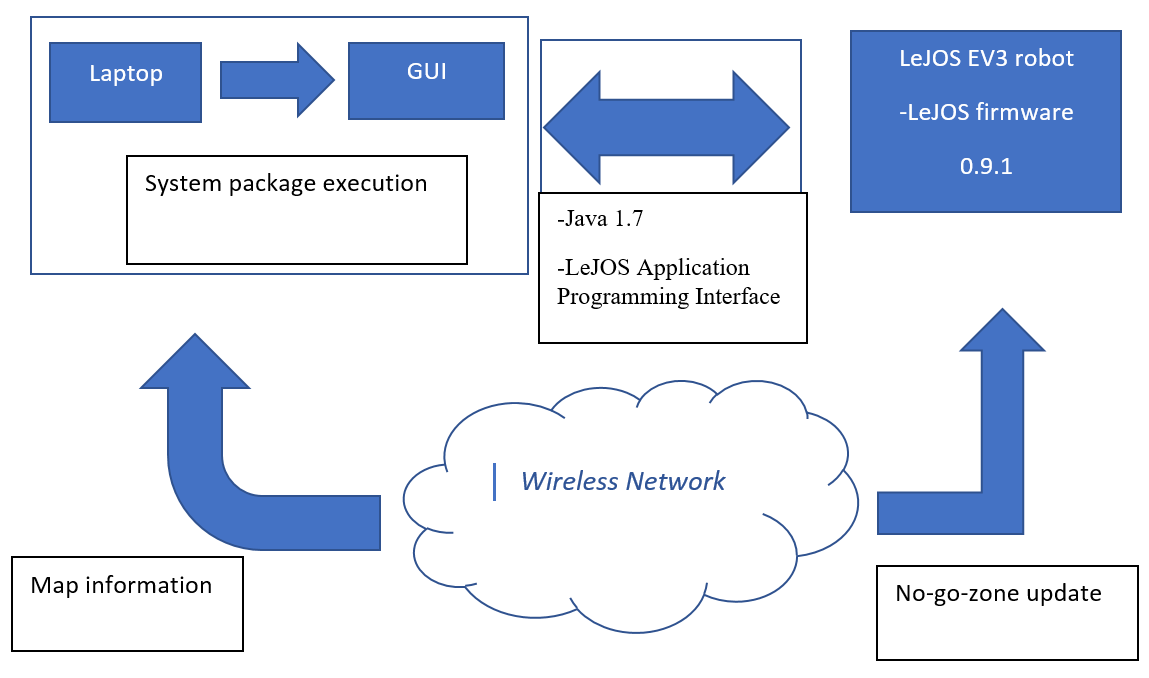
\includegraphics[width=\linewidth]{software_interface.PNG}
		\caption{Flow of software communication}
		\label{fig:Flow of software communication}
	\end{figure}
	
	\subsubsection*{System Package Details}
	- JDK 1.7 development environment.\\
	- LeJOS 0.9.1 library including ev3 classes.\\
	
	These two libraries are for making a jar file which can be executed in LeJOS firmware. Also, ev3 classes provide necessary application programming interfaces for the system to communicate with robot.
	
	\subsubsection*{Software Components}
	\begin{itemize}
		\item LeJOS EV3 is running in Linux and LeJOS EV3 0.9.1 is supporting JAVA 1.7 only.     
		Therefore, the system is developed in JAVA 1.7 environment.
		\item User must execute the system via provided libraries in the system package. System package contains all necessary libraries for running the system.
		\item Robot can be controlled by user via GUI only.
		\item All data and mapping information will be transferred via wireless network. There are 100ms delay. In case of unavailable of wireless network, the system also provides Bluetooth network for communication. However, it is very unstable and is not recommended .
	\end{itemize} 
	
	\subsubsection*{LeJOS Application Interface}
	\begin{itemize}
		\item Manual control
		\item Package: LeJOS.hardware.motor, LeJOS.hardware.port and LeJOS.hardware.sensor
		\item This package of API's is for the system to access robot’s hardware such motor and sensor
		\item Automatic control
		\item Package: LeJOS.robotics.navigation, LeJOS.robotics.pathfinding, LeJOS.robotics.objectdetection, LeJOS.robotics.mapping
		\item This package of API's is for the system to navigate the map and detect the obstacle automatically. Also, the robot will update the map information to the system
		\item The detail about mapping mechanism will provide later
	\end{itemize} 
	
	\subsection{Communications Interfaces}
	The communication including data transfer and API communication is via wireless network (WiFi). The below is the standard for establishing wireless channel and supporting type of communication.
	
	\subsubsection*{LeJOS ev3 robot and remote system communication:}
	\begin{itemize}
		\item The communication channel is established via WiFi.
		\item The Digitech WiFi dongle is used for EV3 to connect wireless network (Support 802.11 b/g/n standards).
		\item The encryption type for accessing wireless network supports WPA2 or none.
	\end{itemize}
	
	\subsubsection*{The type of communication between LeJOS ev3 robot and remote system:}
	\begin{itemize}
		\item All system messages will be transferred to GUI display area only. It will not send any e-mail alerts to user e-mail. For the detail about what will be shown to the GUI display area, please refer to 5.1 user interface.
		\item Except for software message, the User can get the errors message about EV3 robot via SCP only since there are no external server setting in the EV3 robot.
		\item Since all functionalities are developed running remotely, all mapping information and initial map are supposed to upload to user’s PC. There are no need to transfer any document to EV3 robot.
	\end{itemize}
	
	\section{Other Non-Functional Requirements}
	
	\subsection{Performance Requirements}
	\subsubsection*{NFR01: Map Accuracy}
	\paragraph{Priortiy:} High
	\paragraph{Dependencies:} UR01, UR02, UR03, UR04
	\paragraph{Description:} The visual representation of the map shall be as accurate as possible. The various objects and hazards that the robot encounters must be recognised and drawn as soon as the robot encounters them.
	\paragraph{Rationale:} The client must be able to use the map for other purposes once the crash site has been found and therefore is relying on the map to be an accurate representation of the environment. In addition, the robot must be able to use the map to determine where past obstacles were to allow for smooth navigation and to avoid unnecessary travel time.\\
	
	\subsubsection*{NFR02: Speed}
	\paragraph{Priortiy:} Medium
	\paragraph{Dependencies:} None
	\paragraph {Description:} The surveying of the land and discovery of the goal shall be completed in reasonable time. For this prototype, this shall be interpreted as no more than 25 minutes to complete the journey form landing to returning to the landing zone after completing the goal. On manual control this shall be determined by the operator of the robot but will not be allowed to exceed a specified limit for safety purposes.
	\paragraph {Rationale:} The robot will have a limited power supply and must be able to complete its mission before that power runs out. 
	
	\subsection{Safety Requirements}
	\subsubsection*{Significant Impact}
	\paragraph{Priortiy:} High
	\paragraph{Dependencies:} UR09
	\paragraph {Description:} While on autopilot, the robot shall not exceed \begin{math}0.3 m/s\end{math}. When detecting an obstacle, the robot shall stop within 0.15 metres before collision to avoid significant impact and to allow for turning room. During prototype testing, a collision will be deemed significant impact if the robot manages to physically move an obstacle. The manual controller shall default to no more than \begin{math}0.3 m/s\end{math} however the pilot may have additional speed options available to them.
	\paragraph {Rationale:}The safety of any persons on the landing site is paramount and a collision of the actual robot to any persons may lead to severe injury or death. The prototype is also representing a robot that will be expensive to repair and significant damage to the robot may lead to irreparable damage and failure of the mission.
	
	\subsubsection*{NFR03: No Go Zones}
	\paragraph{Priortiy:} High
	\paragraph{Dependencies:} UR10
	\paragraph {Description:} No more than half the robot may enter the NGZ at any time.\\
	\paragraph{Rationale:} An NGZ may represent an area where personnel are active or may indicate an area of known hazardous materials or obstacles otherwise not detectable by the robot. For the safety of the personnel and the robot, the prototype must be able to demonstrate the ability to maneuver its way out of an NGZ without risking injury to personnel or getting stuck in an hazardous area.\\
	
	\subsection{Security Requirements}
	\subsubsection*{NFR04: Unauthorised Access}
	\paragraph{Priortiy:}Medium
	\paragraph{Dependencies:}TBD
	\paragraph {Description:} The GUI shall have a login section where a username and password is presented and verified before the controller can be used.\\
	\paragraph{Rationale:} Unauthorised use of the robot may lead to damage or loss if targeted by malicious competition or an individual who has not been verified by the client.\\
	
	\subsection{Software Quality Attributes}
	
	\subsubsection*{NFR05:Ease of use}
	\paragraph{Priortiy:} Low
	\paragraph{Dependencies:} None
	\paragraph {Description:} The GUI shall have intuitive controls and clearly marked buttons. The size of the controller and map shall be set to a size that is sufficient for comfort and legibility. The visual style of the GUI will conform to the standards of similar controller layouts commonly found in maps and remote controllers.\\
	\paragraph {Rationale:} The Client will have limited time to spend learning controls and must be able to intuitively navigate the GUI without much training. This should include importing and exporting map data.\\
	
	\section{Other Requirements}
	
	\section{Appendix A: Glossary}
	\textbf{GUI:} Graphical User Interface\\	
	\textbf{MJ:} "Michael Jackson" - internal nickname to lunar robot and controller application	\\
	\textbf{NGZ:} No-Go Zone\\
	\textbf{TBD:} To Be Determined\\
	\textbf{UI:} User Interface\\
	
		\section{Appendix B: Analysis Models}
	
	\section{Appendix C: Issues List}
	
\end{document}


